%********** Chapter 6 **********
\chapter{Robot World}\index{Robot World}\index{projects!Robot World}

\section{Introduction}

This chapter presents the Robot World project, which creates a simple, simulated world of robots.  Initially, the world and the robots are fairly primitive, but the program's design makes it fairly easy to make them more complex and interesting.

This chapter reviews a number of topics from  previous chapters, most notably classes and arrays.  In addition, a number of new topics are introduced:
\begin{tight_itemize}
  \item User-defined Libraries\index{libraries!user-defined}
  \item Two-dimensional Arrays\index{arrays!two-dimensional}
  \item Pointers\index{pointers}
\end{tight_itemize}

The previous programs have all included libraries of predefined code, such as the \codefont{iostream} library.  This chapter explains how to create libraries.  Libraries are convenient for breaking a large program into more manageable pieces and make it easy to share classes and functions between programs.   This chapter demonstrates how one-dimensional, list-like arrays can be extended to two-dimensional, table-like, arrays or, more generally, to \emph{N}-dimensional arrays.  Finally, this chapter introduces pointers, a type of variable that gives more direct access to memory.

\section{The Program}

The Robot World program should be separated into three separate files: the main file (Listing~\ref{listing:robotWorldMain}), which can have any name, and two library files: ``robot.h'' (consisting of Listing~\ref{listing:roboth} followed by Listing~\ref{listing:robotcpp}) and ``world.h'' (consisting of Listings~\ref{listing:worldh} followed by Listing~\ref{listing:worldcpp}).  Note that the names of the library files are used in \cf{include} statements in the other files, so can't be changed (unless the \cf{include} statements are also changed).\footnote{Libraries are often divided into two files, a .h file containing the function and class declarations and a separate .cpp file with the code definitions.  This is important for mutually dependent libraries, but for this project we will simplify matters by using only a single library file per class.}  
%To compile the program, put the code from Listing~\ref{fig:robotWorldMain} into one file (as always, don't include the line numbers); this is the main program.  Put the code from Listings~\ref{fig:roboth} and~\ref{fig:robotcpp}, in that order, into a file named ``robot.h'' and put the code from Figures~\ref{fig:worldh} and~\ref{fig:worldcpp}, in that order, into a file named ``world.h''.
%Notice that the main program already contains the code to include these libraries (lines 5 and 6).

Compile the main program. The other files will be included automatically.  Then run the program.  To see the robots move repeatedly, press, or hold down, the Enter key.  Two robots, each represented by a `\#', move around a small world consisting of periods and hyphens.  Text at the bottom of the screen supplies information about the robots' status.  Currently, the robots move randomly and don't interact with their world.  However, the structure of the program makes this relatively easy to change.  The program runs indefinitely, so it's necessary to press \codefont{control-c} to stop it.

\begin{minipage}{\textwidth}
\begin{lstlisting}[language=C++,numbers = left,xleftmargin=4.0ex, basicstyle=\small, emph={a_world},emphstyle = \color{\mycolor},
showstringspaces=false,
caption = {The main program for the Robot World program.  The code to include the libraries containing the \codefont{robot} class and the \codefont{world} class is already part of the main program (lines 5 and 6).},
label={listing:robotWorldMain}]
     #include<iostream>
     #include<cstdlib>
     #include<ctime>
     using namespace std;
     #include"robot.h"
     #include"world.h"
     int main(){
         world a_world;
         srand(time(NULL));
        a_world.set_up();
        do{
            a_world.update();
            a_world.draw();
            cin.ignore();
        }while(1);
        return 0;
    }
\end{lstlisting}
\end{minipage}

%---------------------------------------------------------------------------------------------------------

\begin{minipage}{\textwidth}
\renewcommand*\thelstnumber{\the\value{lstnumber}a}
\begin{lstlisting}[language=C++,numbers = left,xleftmargin=4.0ex, basicstyle=\small, emph={direction,energy,ID,moved},emphstyle = \color{\mycolor},
showstringspaces=false,
caption = {The declaration of the \codefont{robot} class.  It has four private data members, three private member functions, and five public member functions.},
label={listing:roboth}]
    class robot{
       private:
          int direction;
          int energy;
          int ID;
          int moved;  
          void turnLeft();                   // a private function
          void turnRight();                  // a private function
          void forward(int &, int &);        // a private function
      public:
         robot(int);                        
         void refresh() {moved = 0;}        // an in-line function
         void draw();
         void print();
         void move(int &, int &);           // pass-by-reference arguments
   };
\end{lstlisting}
\end{minipage}

\begin{minipage}{\textwidth}
\renewcommand*\thelstnumber{\the\value{lstnumber}b}
\begin{lstlisting}[language=C++,numbers = left,xleftmargin=4.0ex, basicstyle=\small, emph={energy,direction,ID,id,x,y,moved},emphstyle = \color{\mycolor},
showstringspaces=false,
caption = {The definitions of the member functions of the \codefont{robot} class.},
label={listing:robotcpp}]
void robot::turnLeft(){
      energy--;
      direction = (direction + 3) % 4; // a left is 3 rights
}
void robot::turnRight(){
      energy--;
      direction = (direction + 1) % 4;
}
void robot::forward(int &x,int &y){
      energy -= 2;
      if(direction == 0)
           y--;    
      if(direction == 2)
           y++;    
      if(direction == 1)
           x++;    
      if(direction == 3)
           x--;    
}
robot::robot(int id){
     energy = 50;
     ID = id;
     moved = 0;
     direction = 0;
}
void robot::draw(){
     cout << "#";
}
void robot::print(){
     cout<<"ID" <<ID<<": Energy = "<<energy<< "   Direction = "<<direction;
}
void robot::move(int &x,int &y){
     if(moved == 1)
          return;
     switch(rand()%4){
     case 0:
          turnLeft();
          break;
     case 1:
          turnRight();
          break;
     case 2:
     case 3: 
          forward(x,y);
          break;
     default: 
          cout << "Error in robot move." << endl;
     }
     moved = 1;
}
\end{lstlisting}
\end{minipage}

\begin{minipage}{\textwidth}
\renewcommand*\thelstnumber{\the\value{lstnumber}c}
\begin{lstlisting}[language=C++,numbers = left,xleftmargin=4.0ex, basicstyle=\small, emph={HEIGHT,WIDTH,terrain,bots},emphstyle = \color{\mycolor},
showstringspaces=false,
caption = {The declaration of the \cf{world} class.},
label={listing:worldh}]
const int HEIGHT = 10;
const int WIDTH = 10;
class world{
   private:
      int terrain[WIDTH][HEIGHT];
      robot *bots[WIDTH][HEIGHT];
   public:
      void set_up();
      void draw();
      void update();
};
\end{lstlisting}
\end{minipage}

\subsection{Two-Dimensional Arrays}

Two-dimensional arrays are similar to the one-dimensional arrays introduced in the Generic Board Game (Chapter 6) where an array was used to store a list of \codefont{square} objects representing the game board.  Two-dimensional arrays extend the idea of a list of items to a table of items.  In a two-dimensional array, each data item is referred to by its row and column number.
Two sets of square brackets are used to declare two-dimensional arrays and to access their elements.    For example,\\
\codefont{int sample\_array[5][10];}\\
declares a 5 by 10 array of integers.  Element \codefont{i,j} is accessed by the statement:\\
 \codefont{sample\_array[i][j]}\\
This pattern extends to $N$ sets of brackets for $N$-dimensional arrays.  

Because memory is simply one long list, a \codefont{X} by \codefont{Y} array is stored in memory as \codefont{X}  arrays, each of length \codefont{Y}.  To access element \codefont{i,j} of an \codefont{X} by \codefont{Y} array a program starts at the beginning of the array and moves \codefont{i*Y + j} elements ahead.   This means that if an $N$-dimensional array is going to be passed to a function, the function must be given all of the dimensions except the first.  That is the function must be declared like\\
 \codefont{return\_type function\_name(argument\_type array[][Y])}\\
where \codefont{Y} is the size of the array's second dimension.  The size of the first dimension can be included, but it doesn't have to be.  For \codefont{N} dimensional arrays passed as arguments to functions, the size of the last \codefont{N - 1} dimensions must be given.




\begin{figure}
%\centerline{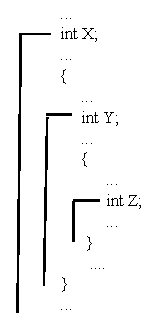
\includegraphics[width=9cm,height=6cm]{images/scope1.eps}}
\setlength{\unitlength}{1cm}
\begin{picture}(10,3)
\linethickness{0.3mm}

\put(2.3,2.5){\codefont{ptr}}

\put(4.3,2.1){\codefont{X}}
\put(4.7,1.6){\codefont{9}}
\color{\mycolor}{
\put(2.5,2.4){\line(1,0){1}}
\put(2.5,1.9){\line(1,0){1}}
\put(2.5,2.4){\line(0,-1){0.5}}
\put(3.5,2.4){\line(0,-1){0.5}}

\put(3.2,2.2){\vector(3,-1){1.2}}

\put(4.5,2.0){\line(1,0){1}}
\put(4.5,1.5){\line(1,0){1}}
\put(4.5,2.0){\line(0,-1){0.5}}
\put(5.5,2.0){\line(0,-1){0.5}}
}

% right side figure
\color{black}{
\put(8.1,2.5){address\hspace*{0.2cm}stored value\hspace*{0.2cm}variable name}
\put(11.8,2){\codefont{ptr}}
\put(11.8,1.0){\codefont{X}}
\put(8.1,2.0){0x7a01\hspace*{0.3cm}7a08}
\put(8.1,1.5){0x7a04}
\put(8.1,1.0){0x7a08\hspace*{0.3cm}9}
\put(8.1,0.5){0x7a0c}
}

\color{\mycolor}{
\put(9.3,2.8){\line(0,-1){2.4}}
\put(11.5,2.8){\line(0,-1){2.4}}
\put(9.3,2.4){\line(1,0){2.2}}
\put(9.3,1.9){\line(1,0){2.2}}
\put(9.3,1.4){\line(1,0){2.2}}
\put(9.3,0.9){\line(1,0){2.2}}
\put(9.3,0.4){\line(1,0){2.2}}
}

\end{picture}
\caption{{\bf Left:} Illustration of a pointer.  The variable \codefont{ptr} is a pointer that ``points'' to (or refers to) the variable \codefont{X}. 
{\bf Right:} Pointers actually work by storing the ``target'' variable's address; for example, \codefont{ptr} stores \codefont{X}'s address: 7a08 (addresses are typically written in hexadecimal).  This allows \codefont{ptr} to access the value of \codefont{X} using the dereference operator: \cf{*} or to pass the address of \codefont{X} to a function.  The ``0x'' before the addresses is used to indicate that the values are written in hexadecimal.  Note that many variable types, including pointers and integers, actually use more than one location (or byte) in memory to store the data.}
\label{fig:pointers1}
\end{figure}

\subsection{Pointers}\index{pointers}

One of the most powerful, most difficult, and most dangerous (in the sense of being likely to cause serious, hard-to-find errors) elements of C++ is \emph{pointers}.  To help understand how pointers work, it is important to understand that every variable is stored somewhere in the computer's memory and that every memory location has an \emph{address}\index{addresses} associated with it.
For example, the statement:\\
\codefont{int X = 9;}\\
sets aside a section of memory\footnote{This section of memory is the ``box'' associated with variables in earlier chapters.} for the variable \codefont{X} and places the value 9 in that section of memory.  Memory addresses are typically written as a hexadecimal (base 16) number such as \codefont{a70b3}.  (Appendix~\ref{appendix:hexadecimal} discusses hexadecimal, and binary, numbers in more detail.)  In C++ an ``0x'' is usually printed in front of the number to indicate that it is hexadecimal; for example, \codefont{0xa70b3} stands for the hexadecimal number \codefont{a70b3}.   A pointer is a variable that holds the \emph{address} of another variable.  You can think of a pointer variable as ``pointing to'' the box of another variable.   Figure~\ref{fig:pointers1} illustrates this idea. 

 A pointer is declared using an asterisk (*):\\
\codefont{int *ptr;}\\
The pointer's name is \codefont{ptr}, and it should point to a variable of type \codefont{int}.
Pointers can be used to point to variables,  objects, or to new `unnamed' data.  Table~\ref{tab:pointers} summarizes the operators that are commonly applied to pointers.

The following snippet of code illustrates the use of pointers:\\
\codefont{
a]   int X = 7;  \hspace{1cm} \textbackslash \textbackslash~create an integer variable \\
b]   int *ptr;   \hspace{1.2cm} \textbackslash \textbackslash~create a pointer variable \\
c]   ptr = \&X;   \hspace{1.2cm} \textbackslash \textbackslash~`point' ptr at X, the \& returns X's address \\
d]   *ptr = 9;  \hspace{1.2cm} \textbackslash \textbackslash~change the value stored in X's `box' \\
e]   cout << X;  \hspace{1cm} \textbackslash \textbackslash~print X, this prints \emph{9} \\
f]   ptr = new int; \hspace*{0.2cm} \textbackslash \textbackslash~ptr points to a new, unnamed, integer instead of X \\
g]   *ptr = 11;  \hspace*{1.0cm} \textbackslash \textbackslash~ptr now points to the value 11, X doesn't change\\
h]  delete ptr; \hspace*{0.9cm} \textbackslash \textbackslash~frees the space that ptr was pointing to\\
}
This code creates a variable named \codefont{X} (line a) and a pointer variable named \codefont{ptr} (line b).  Line c makes  \codefont{ptr} ``point'' to  \codefont{X}.  The ampersand (\&) on line c can be read as ``address of,'' so \codefont{ptr} stores the address of \codefont{X} (as illustrated in Figure~\ref{fig:pointers1}).  

On line d, the asterisk (known as the \emph{dereference}\index{dereference} or \emph{indirection}\index{indirection} operator) can be read as ``box being pointed to,'' so line d changes the value in the box \codefont{ptr} points to a 9.  Because \codefont{ptr} points to the variable \codefont{X} (line c), this means that \emph{the value of \codefont{X} changes from 7 to 9}.  Thus, on line e, the value \emph{9} is printed.  

Pointer variables can be printed directly:
\codefont{cout << ptr;} This will print the address (as a hexadecimal value) stored by the pointer.  In this case, the \emph{address of} \codefont{X}.

The change in \codefont{X}'s value illustrates both the power and risk of pointers.  They give direct access to other variables and to the computer's memory, which is a powerful capability.  However, using pointers can also cause the value of variables to change ``mysteriously''; that is, without it being obvious in the program why a particular value is changing.  

%-------------------------------------------------------------------------------

\begin{minipage}{\textwidth}
\renewcommand*\thelstnumber{\the\value{lstnumber}d}
\begin{lstlisting}[language=C++,numbers = left,xleftmargin=4.0ex, basicstyle=\small, emph={x,y,bots,terrain,tempx,tempy,temp},emphstyle = \color{\mycolor},
showstringspaces=false,
caption = {Definitions of the member functions of the \cf{world} class.},
label={listing:worldcpp}]
void world::set_up(){
     for(int y = 0; y < HEIGHT; y++){
           for(int x = 0; x < WIDTH; x++){
                bots[x][y] = NULL;
                terrain[x][y] = rand()%2;
            }
     }
     bots[2][2] = new robot(1);
     bots[7][7] = new robot(2);
}
void world::draw(){
    for(int y = 0; y < HEIGHT; y++){
          for(int x = 0; x < WIDTH; x++){
               if(bots[x][y] == NULL)
                     cout << (char)(terrain[x][y] + 45);
               else
                     bots[x][y] -> draw();
          }
          cout << endl;
    }
    for(int y = 0; y < HEIGHT; y++)
          for(int x = 0; x < WIDTH; x++)
               if(bots[x][y] != NULL){
                     bots[x][y]->print();
                     bots[x][y]->refresh();	
                     cout << "\n";
               }
}
void world::update(){
    int tempx,tempy;
    robot *temp;
    for(int y = 0; y < HEIGHT; y++){
          for(int x = 0; x < WIDTH; x++){
               if(bots[x][y] != NULL){
                     tempx = x;
                     tempy = y;
                     bots[x][y] -> move(tempx,tempy);
                     if(tempx < 0 || tempx >= WIDTH)
                           tempx = x;
                     if(tempy < 0 || tempy >= HEIGHT)
                           tempy = y;
                     if(bots[tempx][tempy] == NULL){
                           temp = bots[x][y];
                           bots[x][y] = NULL;
                           bots[tempx][tempy] = temp;
                     }  
               }
          }
    }
}
\end{lstlisting}
\end{minipage}

Another important feature of pointers is that they can be used to allocate memory for storing data dynamically.  With variables the programmer must know in advance exactly how much data they need to store and create exactly that many variables.  However, in many applications the amount of data isn't known in advance.  For example, in a chat room type application the programmer won't know how many people might log-in.  Thus, pointers serve an important purpose by allowing the program to dynamically allocate memory.  

In the sample code line f uses the \cf{new} command to allocate memory to store an \cf{int}; that is it creates a new, unnamed, box for an integer and points \codefont{ptr} to it.  So, after line f \codefont{ptr} stores the address of the new box instead of \codefont{X}'s address.  Line g sets the value in the new box to 11.  Line h deletes the box, effectively ``recycling'' that section of memory.  Note that \codefont{ptr} itself isn't deleted and can continue to be used, although it will need to be pointed to a new address.

The \codefont{delete} function is important because otherwise there's no way to ``recover'' memory that was allocated using the \codefont{new} command.  If delete isn't used properly, a long-running program may keep reserving memory with \codefont{new} without releasing it and can potentially run out of memory.  This type of error, where memory is allocated using the \codefont{new} command and is never deallocated\index{memory!deallocation} (or ``freed'') using the \codefont{delete} command, is known as a ``memory leak.''\index{memory leak}\index{errors!memory leak}

\begin{table}
\centering
\caption{Pointer Operators.}
\begin{tabular}{|  c|  p{3.0cm}| p{9.5cm} |}
%\hline
%\bold{Command} & \bold{Full Name} & \bold{Description} \\
%\multicolumn{3}{|c|}{Using the following definitions: } \\
%\multicolumn{3}{|c|}{\codefont{char c\_str[]}} \\
%\multicolumn{3}{|c|}{\codefont{string str1, str2}} \\
%\multicolumn{3}{|c|}{\codefont{int N}} \\
\hline
\textbf{Operator} &  \textbf{Examples} & \textbf{Description} \\
\hline
* &  \codefont{int *p;} \newline \codefont{robot *ptr;} & Used to declare a pointer.  For example, \codefont{p} is a pointer to an \codefont{int} and \codefont{ptr} is a pointer to a \codefont{robot} object.\\ 
\hline
\& & \codefont{p = \&X;} & Returns the \emph{address} of a variable.  \codefont{p} now stores the address of \codefont{X}; i.e., \codefont{p} \emph{points to} \codefont{X}.\\
\hline 
* & \codefont{*p = 7;}\newline \codefont{cout $<<$ *p;} & \emph{Dereferences} a pointer; e.g., follows the pointer to the box it's pointing to.  The box \codefont{p} is pointing to now holds the value 7 and the \codefont{cout} statement will print 7.\\
\hline
\codefont{new} & \codefont{p = new int;} &
Creates a new, unnamed variable of the given type and points the pointer at it (i.e., the pointer stores the address of the new variable).  Variable \codefont{p} points to a new unnamed box capable of storing an integer.\\
\hline
\codefont{delete} & \codefont{delete p;} & Deletes the variable the pointer is pointing to, allowing that piece of memory to be reused.  The variable that \codefont{p} was pointing to is no longer available.  Note that \codefont{p} is still available.\\
\hline
-$>$ & \codefont{ptr-$>$print();} & Accesses a function or data member of the object being pointed to.  The object being pointed to by \codefont{ptr} will run its \codefont{print()} function.  Used like the dot notation, but with pointers to objects.\\
\hline
NULL & \codefont{ptr = NULL;} & NULL acts like a value, not an operator.  It is used to denote a pointer that is not currently pointing at anything.\\
\hline
\end{tabular}\label{tab:pointers}
\end{table}


Pointers can also point to objects.  For example, the following snippet of code illustrates a pointer pointing to an object (of the \cf{pet} class):\\
\codefont{
a]   pet my\_pet; \hspace{1.7cm}  \textbackslash \textbackslash~create a pet object \\
b]   pet *ptr2;  \hspace{1.9cm}  \textbackslash \textbackslash~create a pointer \\
c]   ptr2 = \&my\_pet;  \hspace{0.95cm}  \textbackslash \textbackslash~`point' ptr2 to my\_pet \\
d]   ptr2 -> play(); \hspace{0.9cm}  \textbackslash \textbackslash~use ptr2 to call my\_pet's play() function\\
}
This code creates a pet object called \codefont{my\_pet} (line a), a pointer named \codefont{ptr2} (line b), and points \codefont{ptr2} at \codefont{my\_pet} (line c).  Then it uses the pointer to access \codefont{my\_pet}'s \codefont{play()} member function (line d).  Note that because the pet object is being accessed through a pointer the symbol \codefont{->} is used instead of a dot.

\mysubsubsection{The NULL Pointer}\index{NULL@{\cf{NULL}}}
One of the biggest difficulties with pointers is that they often don't point to a valid location in memory.  For example, when a pointer is first created, when the object a pointer is pointing to is deleted, and when a pointer reaches the end of a list or other data structure, are all cases where a pointer may not be pointing to a valid memory location.  In any of these cases, if the pointer is dereferenced (see Table~\ref{tab:pointers}) without first being pointed to a new, valid memory location, the program is likely to fail.  

The \cf{NULL} value is used for pointers that don't point to a valid location.  A pointer may be assigned the value \codefont{NULL}; for example, with the statement \codefont{ptr = NULL;}.  Then a check against \cf{NULL} can be used to determine if a pointer is pointing to a valid memory location.  For example, code like:
\codefont{if(ptr == NULL)\{\\
\hspace*{0.5cm}// Code if the pointer is pointing to NULL, i.e. not to a valid memory location\\
\}\\
else\{\\
\hspace*{0.5cm}// Code if the pointer is pointing to a valid memory location\\
\}\\
}
allows a program do one thing if a pointer is not currently pointing to a valid location and something else if the pointer is pointing to a valid location.  Note that the \cf{NULL} value is not automatically assigned to pointers, it must be done explicitly in the code.

\mysubsubsection{Arrays and Pointers}

In C++, arrays are maintained using a pointer that points to the beginning of the array's data.  When an array is created:\\
\codefont{
int data[10];\\
}
\codefont{data} is a pointer that points to (i.e., stores the address of) the zeroth array element.  This means that \codefont{type []} and \codefont{type *} can be used \emph{almost} interchangeably.\footnote{There are some differences between them, but they are beyond the scope of this text.}  

When an array is passed as an argument to a function, the location of the array in memory (i.e., a pointer to that location) is passed to the function.  This makes the function call much faster because only a single memory address (the beginning of the array) is copied to the function, instead of the array's entire contents.  It also means that any changes made to the array in the function are persistent because the function is changing the original array elements, not a copy of them.

\mysubsubsection{Using Pointers}

%\begin{wrapfigure}
%{r}{0.5\textwidth} \vspace{-0.3cm} 
%\framebox[\linewidth][l]
%{\parbox{0.95\linewidth}{\codefont{Addresses and Hexadecimal}\index{hexadecimal} \\
%Memory addresses are usually given as \emph{hexadecimal}\index{hexadecimal} (base 16) numbers.  Familiar decimal numbers have a ones place ($10^0$), a tens place ($10^1$), a hundreds place ($10^2$), etc.  Hexadecimal numbers use base 16, so they have a ones place ($16^0$), a sixteens place ($16^1$), a 256s place ($16^2$), etc.  Because the digits only go to 9, hexadecimals use characters for the numbers 10 through 15: a=10, b=11, ..., f=15.

%Thus, the hexadecimal number a7b is:\\ 
%$a*16^2 + 7*16^1 + b*16^0 =\\
%$10*256 + 7*16 + 11*1 = 2715\\
%In C++, hexadecimal numbers are usually printed with a leading ``0x'' to indicate that the number is written in hexadecimal.
%}}
%\vspace{0.0cm} 
%\end{wrapfigure}

Pointers are commonly used for working with large data structures, for creating multiple references to the same data, and for creating dynamic data structures.  Moving large data structures (e.g., passing them to a function or returning them from a function) can be very slow if it requires copying all of the data into, and then back out of, the function's memory.  Instead, a pointer to the data can be used, which avoids having to copy all of the data.  This is another form of pass-by-reference, as a reference to the data, a pointer, is passed to the function instead of the data.  

 Sometimes different segments of a program need access to the same piece of data.  This can be accomplished by having each segment use its own pointer to point to the shared data.

Finally, pointers are often used to create \emph{dynamic} data structures: structures that can allocate and deallocate memory as needed.  Trees, graphs, and other complex data structures are often built dynamically by having each data element in the structure point to one or more other data elements of the structure.  This creates a complex, but often very useful, data structure.  Linked lists, a relatively simple dynamic structure, are presented in Chapter 7.

\section{Analysis of the Code}

In this chapter, the code is analyzed in a \emph{bottom-up} fashion, starting with the basic ``building blocks'' of the program, the \cf{robot} class, then working up to the \cf{world} class, and finishing with the main program.  Looking at the code in this order can be helpful in understanding how all of the pieces fit together.

The program begins by creating a world object in \codefont{main()}.  The world object is a two-dimensional grid of cells represented by two two-dimensional arrays, one keeping track of the world's terrain and the other keeping track of the robots' positions. 
 A loop is used to repeatedly update and print the world.  In each update of the world object, the robots are allowed to move themselves in the world.  

%\subsection{Figures~\ref{fig:roboth} and~\ref{fig:robotcpp}: The Robot Class}

% Each robot has its own energy level, ID number, and a direction its facing.  Each robot also keeps track of whether it has moved yet.  Currently a robot loses energy as it moves, but nothing happens when its energy goes to zero.
%Note that in the robot class three of the functions (\codefont{turnLeft()}, \codefont{turnRight()}, and \codefont{forward()}) are private functions; they can only be called by other members of the robot class.  

\mysubsubsection{Lines 1a-16a: The \cf{Robot} Class Declaration}

The \cf{robot} class defines the code for the robots.  Each robot moves around the simulated world defined by the \cf{world} class.  Each robot has the following data members:
\begin{tight_enumerate}
\item \codefont{direction} - This is an integer that keeps track of the robot's current direction: 0 corresponds to up, which can be thought of as North, 1 to right (East), 2 to down (South), and 3 to left (West).
\item \codefont{energy} - This is an integer that keeps track of the robot's current energy level.  Moving uses energy.  Currently, there is no way to increase energy, and running out of energy has no effect on the robot's behavior.
\item \codefont{ID} - This  integer stores the robot's identification (ID) number.  Currently, it is simply a way to uniquely identify the robots.
\item \codefont{moved} - This integer keeps track of whether a robot has moved in the current time step.  Without it, robots could move multiple times in one time step.
\end{tight_enumerate}

The robot class has three private member functions and five public member functions:
\begin{tight_enumerate}
\item \codefont{turnLeft()} - A private member function that changes the robot's direction to the left, counterclockwise.
\item \codefont{turnRight()} - A private member function that changes the robot's direction to the right, clockwise.
\item \codefont{forward(int \&, int \&)} - A private member function that takes the robot's current position as arguments and calculates the robot's new position based on its current direction.  The arguments are pass-by-reference so that the change to position is persistent.
\item \codefont{robot(int)} - The constructor; it sets the robot's initial energy, direction, and ID.
\item \codefont{refresh()} - This is a public, in-line function (meaning that the code is included in the class declaration) which resets the robot's \codefont{moved} variable.
\item \codefont{draw()} - This function ``draws'' the robot.
\item \codefont{print()} - This function prints data about the robot.
\item \codefont{move(int \&, int \&)} - A public member function that takes the robot's current position as arguments and uses the \codefont{turnLeft()}, \codefont{turnRight()}, and \codefont{forward()} functions to determine the robot's new positions and direction.   The arguments are pass-by-reference, so the change to position is persistent.
\end{tight_enumerate}

\mysubsubsection{Lines 7a, 8a, and 1b-8b: turnLeft() and turnRight()}

The \codefont{turnLeft()} and \codefont{turnRight()} functions allow the robot to turn left and turn right by changing its current direction.  First, these functions subtract 1 from the robot's current energy (lines 2b and 6b), then they change the direction (lines 3b and 7b).  Adding 1 to the direction is equivalent to a clockwise or right turn, then applying a modulus 4 ``wraps'' the value back around to zero if necessary (line 7b).  Subtracting one is a counterclockwise or left hand turn.  However, treating a left hand turn as three right turns makes it possible to use the modulus to ``wrap'' around again. 

\begin{wrapfigure}{r}{0.5\textwidth} \vspace{-0.3cm} \framebox[\linewidth][l]
{\parbox{0.9\linewidth}{\codefont{Pass-by-reference and Pointers}\index{pointers! as arguments} \\
Persistent changes to a function's arguments can be made  using either ampersands (\&'s) or pointers.
For example, the \codefont{forward()} function (line 9b)\\
\codefont{void forward(int \&x, int \&y);}\\
 could be rewritten using pointers as:\\
\codefont{void forward(int *x, int *y);}\\
in which case, the arguments passed to the functions would have to be pointers.  There are two ways to achieve this.  First, the variables passed to the function  could be created as pointers.  In the Robot World program, \codefont{forward()} is called by \codefont{move()} (line 44b), so \codefont{x} and \codefont{y} in \codefont{move()} would need to be pointers.  Alternatively, the variables' \emph{addresses} could be passed to the \codefont{forward()} function.  To do this, the command on line 44b would be changed to\\
\codefont{forward(\&x, \&y);}\\
Then the addresses of \codefont{x} and \codefont{y} would be passed to \codefont{forward()}, where they would be received as pointers, and any changes to them within \codefont{forward()} would persist outside of \codefont{forward()}.
}}
\vspace{-0.5cm} \end{wrapfigure}

Because \codefont{turnLeft()} and \codefont{turnRight()} (and \codefont{forward()}, described next) are all private functions, they can only be called by other members of the robot class.  Currently, they are only called by the \codefont{move()} member function (on lines 37b, 40b, and 44b, respectively).

\mysubsubsection{Lines 9b and 9b-19b: forward()}

The \codefont{forward()} function moves the robot forward.  It takes two integers as arguments, both of which are pass-by-reference (as denoted by the \& symbol in the function declaration and definition)\index{pass-by-reference}\index{arguments!pass-by-reference}.  They represent the \emph{x-y} coordinates of the robot and are pass-by-reference so that they can be changed in the \codefont{forward} function and the change is seen in the calling function (\codefont{move()}).

First, the function removes 2 from the robot's current energy (line 10b) -- moving forward uses more energy than turning.  Next, the program adjusts the \codefont{x} or \codefont{y} value as appropriate for the direction the robot is facing.  
Because  \codefont{x} and \codefont{y} are pass-by-reference, these changes to their values are ``persistent'' and last beyond the scope of the function.  This is necessary because the function could change either \codefont{x} or \codefont{y} and it's not possible to return both values.

\mysubsubsection{Lines 11a and 20b-25b: The Constructor}

The \codefont{robot()} member function is the class's constructor.  It takes a single integer as an argument, which is used to set the robot's ID (line 22b).  The \codefont{robot} constructor also sets the robot's \codefont{energy} to 50 (line 21b), its \codefont{direction} to 0/North (line 24b), and its \codefont{moved} to 0 (line 23b), meaning that it hasn't moved yet this time step.  Note that because capitalization matters \codefont{id}, and \codefont{ID} are different variables.

\mysubsubsection{Line 12a: The \cf{refresh()} Function}

The \codefont{refresh()} function is an \emph{in-line}\index{inline}\index{functions!inline} function, meaning that the function code is defined along with the function declaration (line 15a).  It sets the variable \codefont{moved} to zero, indicating that the robot is ready to move again.  In-line functions often run more efficiently than normal functions, but this depends on how the compiler handles them.  Making a short function that is used very frequently in-line will often improve the overall efficiency of a program.

\mysubsubsection{Lines 12a-13a, 26b-28b, and 29b-31b: The \cf{draw()} and \cf{print()} Functions}

The \codefont{draw()} and \codefont{print()} functions illustrate two different ways a programmer might want to present the robot to the user.  The \codefont{draw()} function ``draws'' the robot on the screen; currently, this just puts a `\#' character at the robot's location.  The
current \codefont{draw()} function can be thought of as a placeholder that could be replaced by a  more interesting function.

 The \codefont{print()} function prints data about the robot: its direction, remaining energy, etc. to the screen.  Notice that although there is only one \codefont{print()} function defined for the robot class, it prints unique information for each of the two robots.  The same function can be applied to either robot, but has different results based on which robot is calling the function.   (The same thing is true of all class member functions, but it's most easily seen with the \codefont{print()} function.)

\mysubsubsection{Lines 12a and Lines 32b-50b: The \cf{move()} Function}

The \codefont{move()} function is used to move the robot; that is, to change the robot's position and/or direction.  It takes two pass-by-reference integers as arguments.   As in the \codefont{forward()} function, the arguments are pass-by-reference so that changes to the \emph{x-y} coordinates of the robot are automatically known by the function that called the \codefont{move()} function, in this case the \codefont{up\_date()} function of a world object.  The \cf{world} object needs to know the new \emph{x-y} position of the robot after it has moved so that it can put the robot in the proper cell in the world (there's no way to return both values, so pass-by-reference is necessary).  

In contrast, the \codefont{turnLeft()} and \codefont{turnRight()} functions don't take any arguments.  The \cf{world} object needs to know the \emph{x-y} coordinates of the robot to place it properly in the world, but it doesn't need to know the direction the robot is facing in (at least not in the current version of the program).  Thus,  there is no need for a pass-by-reference argument to the \codefont{turnLeft()} and \codefont{turnRight()} functions.  

The \codefont{move()} function begins by checking whether the \codefont{moved} variable is equal to 1 (line 33b).  A 1 means that this robot has already moved and should not move again until the next time step.  So, if the value of \codefont{moved} is 1, the function returns without moving the robot.  

Next, a switch statement is used with a random number to choose the robot's next move (line 35b).  The \codefont{rand()} function and modulus operator are used to generate a random number from 0 to 3.  One case goes to \codefont{turnLeft()}, one case to \codefont{turnRight()}, and two cases to \codefont{forward()} (lines 32b and 33b).  This means that the robot is twice as likely to move forward as to turn.  This is not necessary, but it keeps the robot from spending a lot of time turning around in the same spot.  The probability of different robot actions can be changed by adjusting the random values and the number of cases for each action.

A default case is included in the switch (line 46b), even though the default case should never occur (because of the limits on the \codefont{rand()} function).  However, future changes to the code could introduce an error.  If this happens, the default will print an error message and make it easier to identify and fix the problem.  A default case should always be included in a switch statement even if it's not expected to be used.  

Finally, the \codefont{move()} function ends by setting the \codefont{moved} variable to 1, indicating that this robot has now moved and shouldn't move again until the next time step.

%\subsection{Figures~\ref{fig:worldh} and~\ref{fig:worldcpp}: The World Class}

\mysubsubsection{Lines 1c-11c: The World Class Declaration}

The world class defines the ``world'' that the robots move around in, a two-dimensional grid of cells.
   Each cell has its own ``terrain'' and may contain a robot.  Thus, the world class keeps track of two sets of data, the locations of any robots in the world and the terrain:
\begin{tight_enumerate}
\item \codefont{terrain} - A two-dimensional array of ints.  The integer values are used to represent different types of terrain. 
\item \codefont{bots} - A two-dimensional array of \emph{pointers} to robots. 
\end{tight_enumerate}
The world class has fewer, but somewhat more complex functions than the robot class:
\begin{tight_enumerate}
\item \codefont{set\_up()} - This public member function initializes the robot world.
\item \codefont{draw()} - This public member function ``draws'' the robot world.  
\item \codefont{update()} - This public member functions goes through every cell in the world.  If it finds a robot in a cell, it allows that robot to move.
\end{tight_enumerate}

\mysubsubsection{Lines 1c and 2c: The Global Constants}

Lines 1c and 2c define two global constants \codefont{HEIGHT} and \codefont{WIDTH}.  These represent the height and width of the world.  They are constants (as denoted by the keyword \codefont{const} in their definition), meaning that their values can never change when the program is running.  Of course, they can be changed in the programming stage to create a larger, or smaller, world.

\codefont{HEIGHT} and \codefont{WIDTH} are global variables because they are declared before any function (including \codefont{main()}) and outside of any class.\footnote{Global variables are often named in all capitals to make them easy to identify, but this is not a requirement of C++.} This means that their scope extends throughout the program and makes them accessible anywhere in the program without requiring them to be passed as arguments.  For variables that are widely used and never change, making them constant and global can reduce the amount of variable passing required between functions.  Note that it's generally a mistake to make nonconstants global.  Global variables that aren't constants can be changed at too many different places in the code, making it very difficult to keep track of them and easy-to-introduce logical errors.

\mysubsubsection{Lines 5c and 6c: The Data Members}

The world class has two data structures: \codefont{terrain} and \codefont{bots}.  Both of these structures are \codefont{WIDTH} by \codefont{HEIGHT} sized two-dimensional arrays.  The \codefont{terrain} array is an array of integers (line 5c), with different values representing different types of ``terrain'' in the world.

The \codefont{bots} array is an array of pointers to \codefont{robot} objects (line 6c).  The asterisk (*) in the declaration makes it an array of pointers rather than an array of objects, that is the array holds the memory addresses of robot objects rather than the objects themselves.  The \codefont{robot} objects will be created separately using the \codefont{new} command in the \codefont{set\_up()} member function (lines 8d and 9d).

An array of pointers makes sense for several reasons.  First, there are relatively few robots scattered around the ``world.''  So, most of the array elements will be \codefont{NULL}, thus using less memory than if they were mostly ``empty'' robot objects.  Second, as robots move from cell to cell in the world, it's much easier and faster to simply redirect the pointers (lines 44d-46d) than it would be to actually copy the entire \codefont{robot} object from one cell to another.

\mysubsubsection{Lines 8c and 1d-10d: The \cf{set\_up()} Function}

The \codefont{set\_up()} function ``sets up'' the world.  It uses nested \cf{for} loops to initialize every cell in the world (lines 2d-7d).  The outer \cf{for} loop (starting at line 2d) increments through the rows of the world array and the inner \cf{for} loop (starting at line 3d) increments through the columns of the array.  For every value of \codefont{y} from 0 to \codefont{HEIGHT - 1}, the inner \cf{for} loop causes \codefont{x} to count from 0 to \codefont{WIDTH - 1}.  A similar pair of nested \cf{for} loops is used to draw the world (lines 12d and 13d) and to update the world (lines 32d and 33d).  

Initially, all of the pointers in the \codefont{bots} array are set to \codefont{NULL}, indicating that there are no robots in the world (line 4d).   Each terrain cell is set randomly to a value of 0 or 1 (line 5d).  A wider range of terrains could be created by using a wider range of random values.

Lines 8d and 9d create two new robot objects, one at location 2,2 with ID number 1, and one at location 7,7 with ID number 2.  Each robot is pointed to by the respective element of the \codefont{bots} array.  So, the element [2][2] of the \codefont{bots} array points to the robot object with ID number 1, and element [7][7] of the \codefont{bots} array points to the robot object with ID number 2.\footnote{Recall that ``points to'' means that element [2][2] of the \codefont{bots} array stores the memory address where the robot object is stored.}
The \codefont{new} command creates new, \emph{unnamed} robot objects.  Because the objects have no name, they can be accessed only via pointers.

\mysubsubsection{Lines 9c and 11d-28d: The \cf{draw()} Function}

The \codefont{draw()} member function ``draws'' the world (actually printing a two-dimensional array of characters representing the terrain and the locations of the robots), has each robot print itself (line 24d), and reset its \codefont{moved} variable (line 25d).   

To draw the world, the \codefont{draw()} member function uses a pair of nested loops (lines 12d and 13d) to iterate through each cell in the world array.  As the program iterates through the array, it checks whether there is a robot in a given cell (line 14d) by checking if the pointer is equal to \codefont{NULL}.  If the pointer is \codefont{NULL}, it means that there is no robot in that cell, and the function prints the terrain (line 15d) by adding 45 to the value and printing it as a character.  This turns the values 0 or 1 into the character `-' or `.'.

If the pointer is not \codefont{NULL}, it means that a robot is present and the function calls that robot's \codefont{draw()} function (line 18d).  This allows the robot to draw itself in the correct location in the world.  Note how the robot object's \codefont{draw()} function is called:\\
\codefont{bots[x][y] -> draw();} is used, instead of\\
\codefont{bots[x][y].draw();}\\
The arrow (\codefont{->}) notation is used because the array \codefont{bots[][]} stores \emph{pointers} to robot objects instead of actual robot objects.  Whenever a member of an object is accessed via a pointer, the arrow notation is used instead of the dot notation.

%Note that because there is a single command for the if condition (line 15d) it does not need to be surrounded by curly braces.  Similarly because there is a single command for the else condition (line 17d) it does not need to be surrounded by curly braces.  Although the curly braces are not necessary it is often better to include them for clarity and in case extra lines are added to either of those conditions in future revisions of the program.  They are omitted here as both an illustration of when they are not necessary and to save some space in the code (which is not normally a consideration).

 Line 19d adds a new line after each row of the map so that the world is drawn as a grid rather than a single long line.

Next, the \codefont{draw()} function iterates through the \codefont{bots[][]} array a second time (lines 21d and 22d) and has the robots print themselves (line 24d) and then refresh themselves (line 25d).  Again, the arrow notation is used because the \codefont{bots[][]} array holds pointers to robot objects, not the robot objects themselves.
Printing has to be done as a separate set of loops from drawing so the robot data is printed below the world grid instead of in the middle of it.  In the \codefont{refresh()} function, the robot resets its \codefont{moved} variable back to 0 so it is ready to move again.

\mysubsubsection{Lines 10c and 29d-50d: The \cf{update()} Function}

The role of the \codefont{update()} function is to go through the ``world'' and have each robot move itself, keeping track of the robots' new locations.   Line 30d declares two integer variables that are used to temporarily store the location of a robot.  Line 31d declares a pointer to a robot.  Note that this does not create a new robot object; it simply creates a pointer that \emph{can be} used to point to a robot object.

Lines 32d and 33d define a pair of nested \cf{for} loops that go through all of the elements of the \codefont{bots[][]} array.  For each element of the array that is pointing to a bot object (i.e., is not \codefont{NULL} (line 34d)) the function has that bot object move itself.  

First, the function stores the current location of the bot (lines 35d and 36d).  Then the function calls the bot's \codefont{move()} function, passing the temporary \emph{x} and \emph{y} values as arguments.  These arguments are pass-by-reference, so when the \codefont{move()} function is finished, the values of the arguments (\codefont{tempx} and \codefont{tempy}) have changed to represent the location the robot is \emph{trying} to move to. 

Lines 38d-41d check whether the new location that the robot is trying to move to is off the edge of the world.  If it is, then the temporary values are set back to the original values (lines 39d and 41d).  So, the robot doesn't move.  

Line 42d checks whether the new location the robot is trying to move to already contains a robot by checking whether the pointer at the new location is \codefont{NULL}.  If it is not \codefont{NULL}, then there is another robot in the way.  The temporary \emph{x} and \emph{y} values are reset to their initial values so the robot doesn't move.

If the pointer at the new location is \codefont{NULL}, then the function sets the pointer \codefont{temp} to point to the robot that's moving (line 43d).  The pointer at the robot's old location is then set to \codefont{NULL} (line 44d), effectively erasing the robot from the world, but not from memory because \codefont{temp} is still pointing to it. Finally, line 45d makes the pointer at the new location point to the robot, adding it back to the world at its new location.  Note that the member data of the robot object (the data for its energy, direction, etc.) was not moved or copied.  Only which pointer in the \codefont{bots[][]} array that was pointing to the robot object changed.  
For example, the program moves a robot at location \codefont{bots[5][4]} to location \codefont{bots[5][5]} by pointing the \codefont{bots[5][5]} pointer to the robot and the pointing the \codefont{bots[5][4]} pointer to \codefont{NULL}.

\subsection{Figure~\ref{listing:robotWorldMain}: The \cf{main()} Function}

Figure~\ref{listing:robotWorldMain} gives the code for the \codefont{main()} program.  Note that it is actually quite short because almost all of the work is done within the classes.  All \codefont{main()} needs to do is create a \cf{world} object and then repeatedly have the world update and print itself.  

\mysubsubsection{Lines 1-6: \#includes}

The standard included libraries (lines 1-3) and the \codefont{using namespace std} command (line 4) are used.  The two new, programmer-created, libraries are included on lines 5 and 6.  The files ``robot.h'' and ``world.h'' should contain all of the \cf{robot} class code and all of the \cf{world} class code respectively.  

%The order these two libraries are included in is important.  The \cf{world} class uses the \cf{robot} class, thus the \cf{robot} class must be included first.  If the two classes were mutually dependent (i.e. \cf{world} used \cf{robot} and \cf{robot} used \cf{world}), then the files would have to be further broken up into separate files for the class declarations and the class definitions. 

\mysubsubsection{Lines 8-10: Initializing the Program}

Line 8 creates one object of type \cf{world} called \codefont{a\_world}.  This object represents the ``world'' that the robots will move around in.  Line 9 seeds the random number function using the current time.  Line 10 calls the \codefont{set\_up()} member function of the \cf{world} class, which initializes the world by generating random terrain and placing the initial two robots.  

\mysubsubsection{Lines 11-15: The Main Program Loop}

Lines 11 and 15 define the main program loop.  One iteration of the loop represents one time step in the robot world. During each iteration, each robot is allowed to make one move.  The condition for the loop is a 1 (line 15).  Because a 1 is always true, this is an infinite loop -- the only way to get the program to halt is to interrupt it using \codefont{control-c}.  Normally, this is not advisable, but in this case it's better than asking the user if he or she wants to continue after every time step.  

Within the loop, the world is updated (line 12).  This is when all of the robots move.  Then the updated world is redrawn (line 13).  This is also when the robots reset their \codefont{moved} variable, allowing them to move again during the next iteration/time step.  Finally, line 14 pauses the program until the user presses the Enter key, which allows the user to track the robots' movements.  The user can also simply hold down the Enter key, in which case the iterations fly by.  


\vspace{+0.25cm}
{\color{\mycolor}\noindent\hrulefill}
\section{Exercises: Modifying the Program}

The Robot World program lends itself to many changes and additions.  The following are just a few of the changes that are interesting and not too complex to implement.  

\mysubsubsection{Exercise 1: World Size} 
Modify the size of the world by changing the variables \codefont{WIDTH} and \codefont{HEIGHT}.  If the \codefont{HEIGHT} variable is set to just under the height of the window the program is running in, it gives the appearance of a continually changing grid (rather than one that's scrolling up the screen).

\mysubsubsection{Exercise 2: More Robots}
Increase the number of robots by adding more \codefont{new robot} commands to the \codefont{set\_up()} member function in the \cf{world} class (lines 8d and 9d).  Each new robot must be added at a different location.  Note that one of the limitations of the program is that there can only be one robot per cell because the pointers in the \codefont{bots[][]} array can point to only one robot.  So, don't try to put more than one robot in a cell.

\mysubsubsection{Exercise 3: Robots with Different Appearances}
Currently, robots are printed as just the character \# (line 27b).  Create a fancier output by using a switch statement to draw a symbol indicating the robots' direction; for example by using the characters: $<$, $\wedge$, $>$, and  $\vee$.  The beginning of the switch statement (replacing line 27b) would look like this:\\
\codefont{
switch(direction)\{\\
case 0:  \\
\hspace*{1cm} cout << "$\wedge$";\\
\hspace*{1cm} break; \\
case 1: \\
\hspace*{1cm} cout << ">";\\
\hspace*{1cm} ...\\
}

\mysubsubsection{Exercise 4: Different Behaviors}
Change the behavior of the robots by modifying the probabilities of picking different actions in the \codefont{move()} member function (lines 35b-48b).  Doing this can make it more likely that the robots move forward by having a wider range of random numbers (line 35b) and more cases associated with moving forward (lines 42b and 43b).

\mysubsubsection{Exercise 5: Different Terrain}
Increase the number of terrain ``types'' by changing line 5d.  Then use a switch statement (in the place of line 15d) to pick the characters that are printed for different terrains.  For example, a switch statement could be used to print \_'s for cells whose value represents plains, T's for cells whose value represents trees, etc.

%Currently the \codefont{energy} variable doesn't do anything except get lower as the robots move.  The \codefont{move()} member function of the robot class could be modified to take the energy into account.  For example, not moving if the energy reaches zero.  Even better the \codefont{move()} function could return a value indicating that the robot is out of energy, allowing the world object to delete it.

\section{Problems}

\begin{enumerate}[{\bf 1.}]
\item {\bf User-controlled robots}\\ 
Currently, the robots move randomly.  Make a new member function of the robot call that asks the user for input to direct the robots.  Have one of the robots call the new function instead of the current \cf{move()} function, allowing a player to control one of the robots.%This could lead to games with two (or more) players, in which the players take turns moving their robot.

\item {\bf Terrain effects}\\
 Currently, the terrain has no effect on how the robots move.  Modify the program so that terrain determines the amount of energy used during a move.  Making this work is a bit tricky.  In the \codefont{up\_date()} member function after a robot moves (around line 44d), the program would need to check the terrain in the robot's new cell (e.g., at \codefont{tempx},\codefont{tempy}) and modify the robot's energy accordingly.  This requires creating a new robot member function that decreases the robot's energy by the amount of the function's argument that is called by the \codefont{up\_date()} function after the robot moves into a new cell.

\item {\bf Other terrain effects}\\
Make some of the terrain impassable, robot's can't move into it.  Make other terrain ``deadly,'' a robot moving into deadly terrain is deleted.  Make a third category of terrain representing vortexes, a robot in this terrain faces in a new random direction.

\item {\bf Energy and terrain}\\ 
Modify the program so that the robot stops moving when it runs out of energy.  This simply requires an additional test in the \codefont{move()} function (line 32b) to make sure that there is sufficient energy left. Now, the robots need a way to gain energy.  Change the program so that moving into some types of terrain gives a robot energy.  This requires a change in the \codefont{up\_date()} function (around line 44d) to check the new terrain and a new function in the \cf{robot} class that is used to change the energy level (see the previous problem).

\item {\bf Changing terrain}\\
 Make the terrain change over time and when a robot moves into it.   Changes over time can be accomplished by defining a new function in the \cf{world} class that uses nested loops to iterate through the \codefont{terrain[][]} array and, with some low probability, changes the existing terrain.
For robot driven changes  the \codefont{update()} function in the \cf{world} class can change the value of a cell in the \codefont{terrain[][]} array if a robot moves into that cell.  

\item {\bf More complex output}\\
Currently, each cell in the world is represented by a single character.  This gives some flexibility in how terrain and robots are ``drawn'' but it is still fairly limited.  Change the program so that each cell is represented by a 2 x 2, 3 x 3, or larger grid of characters when it's printed.  Now have the program draw more complex arrangements of characters in each cell to represent the terrain.  Because the output can only be written one row of characters at a time, this change requires making several print ``passes'' for each row in the world.  

\item {\bf Other variables}\\
 The \codefont{energy} variable was included to illustrate the possibility of robots having ``internal'' data.  Add another variable, like ore or water, that is tied to entering specific terrain.  Some cells should increase the new variable's value and other cells should decrease it.  Modify the \cf{print()} function to also print the value of the new variable, and make sure to comment the code to make it clear what the new variable represents.

\item {\bf Robot interactions}\\
 Currently, when a robot tries to move into another robot's cell, nothing happens except that the robot doesn't move.  Change the code so robots can interact with each other.  Multiple robots can't occupy the same cell, so do one of the following: when a robot tries to move into another robot, one of the two robots is destroyed; or one of the two robots gives energy to the other robot.

\item {\bf File input}\\
 Currently, the world is generated randomly each time the program is run.  Modify the program so that the world is loaded from a file.  This makes it possible to create more realistic worlds, with well-defined areas of different terrain, and to save and reload particular worlds.

\item {\bf Multiple worlds}\\
 Because \cf{world} is defined as a class, it's simple to create multiple worlds by creating multiple objects of type \cf{world}.  Create at least two \cf{world} objects and have particular cells in each world that automatically transport robots to the other world.

\item {\bf Challenge: Pet world}\\
Create a Pet world by modifying the \cf{world} class to point to \cf{pet} objects instead of \cf{robot} objects.  The \cf{pet} class will need to be expanded so that the pets have a \cf{move()} function.  Allow the player to control the pets' movement (see Problem 1) and have special terrain cells that allow the pets to be fed, played with, etc.  For example, if the user moves a pet onto a cell with a particular terrain, the pet automatically calls its \cf{feed()} function.  By arranging the terrain cells in a particular pattern you can create a pet environment with food bowls, play areas, etc.

\end{enumerate}

%Multiple Robot Types

%Duplicating Robots: arrays of robots

%Different control strategies

% multiple worlds?